%% FEUP THESIS STYLE for LaTeX2e
%% how to use feupteses (portuguese version)
%%
%% FEUP, JCL & JCF, 31 Jul 2012
%%
%% PLEASE send improvements to jlopes at fe.up.pt and to jcf at fe.up.pt
%%
%%
%% Adaptation to be used in ISEP (formally authorized by the authors) made by João Araújo 1140570@isep.ipp.pt and Vitor Sousa 1140348@isep.ipp.pt
%%
%% You should note that:
%%%
%% * If you need to use SI units you should use the \SI{}{} command as shown in the example \SI{1250}{\kilo\meter\per\hour}. To use other units please check 'Adenda-SI units' available inside the project.
%%
%% * To use acronyms correctly you need to go to 'Preamble/acronyms.tex' file and add the acronym as shown in the example \addacronym{LSA}{Laboratório de Sistemas Autónomos}. The acronyms are automatically sorted in alphabetical order.
%%
%% * To use keywords correctly you need to add English and Portuguese keywords in the keywords area below in this file. The English and Portuguese keywords are automatically displayed in Abstract and Resumo, respectively.
%%
%% * To add new Figures you just need to put them inside the 'Figures' folder and when you want to "call" it you just need to use the figure name. You do not need to put the path 'Figures/puzzle', only the figure name!
%%
%%% * For other questions about the template adaptation to be used in ISEP please send an email to 1140570@isep.ipp.pt :)


%%========================================
%% Commands: pdflatex tese
%%           bibtex tese
%%           makeindex tese (only if creating an index)
%%           pdflatex tese
%% Alternative:
%%          latexmk -pdf tese.tex
%%========================================

%%----------------------------------------
%% Important Packages
%%----------------------------------------
\documentclass[11pt,a4paper,twoside,openright]{report}
\usepackage[portugues]{feupteses}
%% Options: 
%% - portugues: titles, etc in portuguese
%% - onpaper: links are not shown (for paper versions)
%% - backrefs: include back references from bibliography to citation place
%% - numericrefs: include (numeric) plain references style
%% - alpharefs: include alpha references style

\usepackage[utf8]{inputenc}
\usepackage{siunitx} %SI units
\usepackage{amsmath} % \begin{equation*}
\sisetup{binary-units = true, per-mode=symbol} %SI units setup
\usepackage{graphicx,graphics,float}
\usepackage{enumitem}
% Acronyms
\usepackage{upgreek}
\usepackage{datatool}
\usepackage{acronym}
\usepackage{longtable,multirow,booktabs}

\usepackage{chngcntr}
\counterwithout{figure}{section}
\counterwithout{figure}{subsection}
\counterwithout{table}{section}
\counterwithout{table}{subsection}
%%----------------------------------------
%% Information about the work
%%----------------------------------------
\title{UAV Command Forwarder}
\author{João Pedro Mesquita Azevedo}
\school{Instituto Superior de Engenharia do Porto}
\department{Departamento de Engenharia Eletrotécnica}
\degree{Mestrado em Engenharia Eletrotécnica e de Computadores}
\area{Área de Especialização em Telecomunicações}
\requirements{Este relatório satisfaz, parcialmente, os requisitos que constam da Ficha de Unidade Curricular de Tese/Dissertação, do 2.º ano do Mestrado em Engenharia Eletrotécnica e de Computadores.}

%%----------------------------------------
%% Dates (appear in title pages)
%%----------------------------------------
%\thesisdate{Porto, DAY de MONTH de YEAR}
\thesisdate{Porto, março de 2019}
\thesisyear{2019}

%%----------------------------------------
%% Copyright text
%%----------------------------------------
\copyrightnotice{João Azevedo, 2019} % Comment if not used % Comment if not used

%%----------------------------------------
%% Keywords (appear in abstract)
%%----------------------------------------
% English Keywords
\keywords{Uav, Drones, Networks, Control, Extend, Mesh, Multi-Hop, Routing}
% Portuguese Keywords
\keywordsPT{UAV, Drones, Redes, Controlo, Alcance, Mesh, Multi-hop, Encaminhamento} 

%%----------------------------------------
%% Macros
%%----------------------------------------
%% TIP: if you want to define more macros, use the mymacros file to keep them
%some macro definitions

% format
\newcommand{\class}[1]{{\normalfont\slshape #1\/}}

% entities
\newcommand{\Feup}{Faculdade de Engenharia da Universidade do Porto}

\newcommand{\svg}{\class{SVG}}
\newcommand{\scada}{\class{SCADA}}
\newcommand{\scadadms}{\class{SCADA/DMS}}


%%----------------------------------------
%% Figures directory
%%----------------------------------------
%% TIP: use folder 'Figures' to keep all your figures
\graphicspath{{Figures/}}

%%----------------------------------------
%% PDF identification
%%----------------------------------------
\makeatletter
\AtBeginDocument{
\hypersetup{pdftitle=\@title}
\hypersetup{pdfauthor=\@author}
\hypersetup{pdfkeywords=\@keywords}}
\makeatother

%%========================================
%% Start of document
%%========================================
\begin{document}

%%----------------------------------------
%% Candidate and supervisors info
%%----------------------------------------
\candidate{Candidato}{João Pedro Mesquita Azevedo, \href{mailto:1111476@isep.ipp.pt}{1111476@isep.ipp.pt}}

\supervisor{Orientação científica}{Jorge Botelho Da Costa Mamede, \href{mailto:jbm@isep.ipp.pt}{jbm@isep.ipp.pt}}

%\company{Empresa}{Nome da Empresa}

%\companysupervisor{Supervisão}{Nome do Supervisor Empresa, \href{mailto:YYY@empresa.com}{YYY@empresa.com}}

%%----------------------------------------
%% Signature
%%----------------------------------------
% Uncomment signature line in the final on paper version if used
%\signature 

%%----------------------------------------
%% ISEP Logo
%%----------------------------------------
% Specify cover logo (in folder ``figures'')
\logo{ISEP_logo} 

%%----------------------------------------
%% Preparation of Dissertation (if)
%%----------------------------------------
% Uncomment for additional text below the author's name (title page)
%\additionalfronttext{Preparação da Dissertação} 

%%----------------------------------------
%% Preliminary materials
%%----------------------------------------
% remove unnecessary \include{} commands
\begin{Prolog}
   \cleardoublepage
\thispagestyle{plain}

\vspace*{8cm}

\begin{flushright}
   \textsl{``You should be glad that bridge fell down. \\
           I was planning to build thirteen more to that same design''} \\
\vspace*{1.5cm}
           Isambard Kingdom Brunel
\end{flushright}
    % initial quotation if desired
   \chapter*{Agradecimentos}
%\addcontentsline{toc}{chapter}{Agradecimentos}

Em primeiro lugar de deixar um agradecimento especial com carinho aos meus pais e irmãos, pela força que me deram durante todo este percurso e também pelo esforço por eles feito durante este meu percurso.

Ao resto da família por estarem lá sempre que foi necessário.
Agradecer também aos amigos que estiveram presentes não só nas fases mais fáceis, mas também nas fases mais difíceis, sempre com um gesto animador, em especial ao Adriano Valadar.


A todos os profissionais do ISEP, deixo os maiores agradecimentos pelos conhecimentos transmitidos durante todo o percurso não só na licenciatura como no Mestrado de Engenharia Eletrotécnica e de Computadores – ramo de Telecomunicações. 
Quero também agradecer em especial ao meu orientador científico o engenheiro Jorge Mamede, pela orientação, disponibilidade e ajuda na concretização deste projeto.
 
As recordações dos momentos passados no ISEP, serão para sempre lembradas como uma excelente parte da minha vida.


\vspace{10mm}
\begin{flushleft}
João Pedro Mesquita Azevedo
\end{flushleft}
  % the acknowledgments
  \chapter*{Resumo}
%\addcontentsline{toc}{chapter}{Resumo}

A manutenção de veículos aéreos não tripulados, em inglês UAV, depende em grande parte do controlo remoto. O alcance da operação é limitado pelo sucesso das comunicações via rádio entre o controlador e o UAV. De modo a expandir esse alcance, podem ser utilizadas redes ou enxames de UAVs de modo a definir uma \textit{mesh} com o objetivo de se poder encaminhar comandos de controlo para unidades mais distantes.

Devido aos obstáculos naturais e artificiais que existem no nosso meio ou então devido a interferências intencionais, a comunicação entre os drones é suscetível a interrupções e nesse sentido, é necessário criar soluções que consigam optimizar a comunicação evitando ao máximo as interrupções que possam ocorrer devido aos obstáculos.

Ao longo desta tese é proposta uma especificação, desenvolvimento e teste de um protocolo de sobreposição para encaminhar instruções do controlador para comandar um UAV remoto numa base \textit{multi-hop}.\newline 

\noindent\textbf{Palavras-Chave:. }%\newline\indent
\makeatletter
\@keywordsPT
\makeatother % the PT abstract
  \chapter*{Abstract}
%\addcontentsline{toc}{chapter}{Abstract}

The maintenance of unmanned aerial vehicles, commonly called UAV, depends on the remote control. The scope of operation is limited by the success of radio communications between the controller and the UAV. In order to expand this range the UAVs networks or swarms can be used in order to define a mesh so that control commands can be routed to more distant units.

Due to the natural and artificial obstacles that exist in our environment or intentional interference, communication between the drones is susceptible to interruptions. In this sense is necessary to create solutions that optimize the communication avoiding as far as possible the interruptions that can occur due to those obstacles.

Throughout this thesis it is proposed a specification, development and testing of an overlay protocol to route controller instructions to command a remote UAV on a multi-hop basis.\newline 

\noindent\textbf{Keywords: }%\newline\indent
\makeatletter
\@keywords
\makeatother % the abstract
  \cleardoublepage
  \pdfbookmark[0]{Conteúdo}{contents}
  \tableofcontents
  \cleardoublepage
  \pdfbookmark[0]{Lista de Figuras}{Figures}
  \listoffigures
  \cleardoublepage
  \pdfbookmark[0]{Lista de Tabelas}{tables}
  \listoftables
  \cleardoublepage
  \chapter*{Acrónimos}
\chaptermark{Acrónimos}
% Acronyms autommatically appear by alphabetic order
\DTLnewdb{acronyms}
\begin{acronym}[CDA]
\addacronym{ISEP}{Instituto Superior de Engenharia do Porto}
\addacronym{LSA}{Laboratório de Sistemas Autónomos}
\addacronym{UAV}{\textit{Unmanned Aerial Vehicle}}
\addacronym{ROS}{\textit{Robot Operating System}}
\addacronym{VTOL}{\textit{Vertical Take-Off and Landing}}
\addacronym{UGV}{\textit{Unmanned Ground Vehicle}}
\addacronym{AG}{Genetic Algorithm}
\addacronym{MPC}{\textit{Model Predictive Control}}
\addacronym{LSA}{Laboratório de Sistemas Autónomos}
\addacronym{MEEC}{Mestrado em Engenharia Eletro}
\addacronym{UAV}{\textit{Unmanned Aerial Vehicle}}
\addacronym{ROS}{\textit{Robot Operating System}}
\addacronym{VTOL}{\textit{Vertical Take-Off and Landing}}
\addacronym{UGV}{\textit{Unmanned Ground Vehicle}}
\addacronym{MPC}{\textit{Model Predictive Control}}
\addacronym{LSA}{Laboratório de Sistemas Autónomos}
\addacronym{UAV}{\textit{Unmanned Aerial Vehicle}}
\addacronym{ROS}{\textit{Robot Operating System}}
\addacronym{VTOL}{\textit{Vertical Take-Off and Landing}}
\addacronym{UGV}{\textit{Unmanned Ground Vehicle}}
\addacronym{MPC}{\textit{Model Predictive Control}}
\addacronym{PID}{\textit{Proportional–Integral–Derivative}}
\addacronym{IMU}{\textit{Inertial Measurement Unit}}
\addacronym{USV}{\textit{Unmanned Surface Vehicle}}
\addacronym{UGV}{\textit{Unmanned Ground Vehicle}}
\addacronym{PID}{\textit{Proportional–Integral–Derivative}}
\addacronym{IMU}{\textit{Inertial Measurement Unit}}
\addacronym{USV}{\textit{Unmanned Surface Vehicle}}
\addacronym{UGV}{\textit{Unmanned Ground Vehicle}}
\addacronym{PID}{\textit{Proportional–Integral–Derivative}}
\addacronym{IMU}{\textit{Inertial Measurement Unit}}
\addacronym{USV}{\textit{Unmanned Surface Vehicle}}
\addacronym{UGV}{\textit{Unmanned Ground Vehicle}}
\addacronym{UAV}{\textit{Unmanned Aerial Vehicle}}
\addacronym{ROS}{\textit{Robot Operating System}}
\addacronym{VTOL}{\textit{Vertical Take-Off and Landing}}
\addacronym{UGV}{\textit{Unmanned Ground Vehicle}}
\addacronym{MPC}{\textit{Model Predictive Control}}
\addacronym{PID}{\textit{Proportional–Integral–Derivative}}
\addacronym{IMU}{\textit{Inertial Measurement Unit}}
\addacronym{USV}{\textit{Unmanned Surface Vehicle}}
\addacronym{UGV}{\textit{Unmanned Ground Vehicle}}
\addacronym{PID}{\textit{Proportional–Integral–Derivative}}
\addacronym{IMU}{\textit{Inertial Measurement Unit}}
\addacronym{USV}{\textit{Unmanned Surface Vehicle}}
\addacronym{UGV}{\textit{Unmanned Ground Vehicle}}
\addacronym{PID}{\textit{Proportional–Integral–Derivative}}
\addacronym{IMU}{\textit{Inertial Measurement Unit}}
\addacronym{USV}{\textit{Unmanned Surface Vehicle}}
\addacronym{UGV}{\textit{Unmanned Ground Vehicle}}
\addacronym{IMU}{\textit{Inertial Measurement Unit}}
\addacronym{USV}{\textit{Unmanned Surface Vehicle}}
\addacronym{UGV}{\textit{Unmanned Ground Vehicle}}
\addacronym{UAV}{\textit{Unmanned Aerial Vehicle}}
\addacronym{ROS}{\textit{Robot Operating System}}
\addacronym{VTOL}{\textit{Vertical Take-Off and Landing}}
\addacronym{UGV}{\textit{Unmanned Ground Vehicle}}
\addacronym{MPC}{\textit{Model Predictive Control}}
\addacronym{PID}{\textit{Proportional–Integral–Derivative}}
\addacronym{IMU}{\textit{Inertial Measurement Unit}}
\addacronym{USV}{\textit{Unmanned Surface Vehicle}}
\addacronym{UGV}{\textit{Unmanned Ground Vehicle}}
\addacronym{PID}{\textit{Proportional–Integral–Derivative}}
\addacronym{IMU}{\textit{Inertial Measurement Unit}}
\addacronym{USV}{\textit{Unmanned Surface Vehicle}}
\addacronym{UGV}{\textit{Unmanned Ground Vehicle}}
\addacronym{PID}{\textit{Proportional–Integral–Derivative}}
\addacronym{IMU}{\textit{Inertial Measurement Unit}}
\addacronym{USV}{\textit{Unmanned Surface Vehicle}}
\addacronym{UGV}{\textit{Unmanned Ground Vehicle}}
\addacronym{ISEP}{Instituto Superior de Engenharia do Porto}
\addacronym{INESC TEC}{Instituto de
Engenharia de Sistemas e Computadores, Tecnologia e Ciência}
\addacronym{OET}{Tecnologias Óticas e Eletrónicas (\textit{Optical and Electronic Technologies})}
\addacronym{UOWC}{Comunicações óticas sem fios subaquáticas (\textit{Underwater Optical Wireless Communication})}
\end{acronym}
\DTLsort{Acronym}{acronyms}

\begin{longtable}{m{2.2cm}m{12.2cm}}
\DTLforeach*{acronyms}{\thisAcronym=Acronym,\thisDesc=Description}{
\hspace{-0.4cm}\textbf{\thisAcronym} & \thisDesc\\[5pt]1}
\end{longtable}
  % the list of abbreviations used
\end{Prolog}

%%----------------------------------------
%% Body
%%----------------------------------------
\StartBody

%% TIP: use a separate file for each chapter
%%
\chapter{Introdução} \label{chap:intro}

\section{Contexto} \label{sec:context}

Os \textit{drones}, ou veículos aéreos não tripulados, vêm cada vez mais a ser uma realidade nos dias que correm. A sua área de atividade é bastante extensa e tem vindo a emergir em diversos níveis, tanto a nível civil como a nível militar, incluindo escoltas militares, troca de mercadorias em algumas cidades, gestão do trânsito, fotografia aérea, segurança urbana e por aí adiante \cite{8255738}. Devido aos obstáculos naturais que podem existir nos diferentes cenários descritos em cima ou então por interferências intencionais, a comunicação entre os UAVs é suscetível a interrupções \cite{Secinti2018} e nesse sentido, é necessário encontrar medidas para tornar a comunicação mais eficiente.

Com o advento das tecnologias robustas das redes \textit{wireless}, os UAVs equipados com \textit{transceivers} podem ser habilitados para comunicar com os nós terrestres assim como os outros UAVs \cite{Morgenthaler2012a}. Deste modo é possível um comando qualquer da estação possa chegar a unidades cada vez mais remotas.

Com o progresso dos sistemas embebidos e a tendência para a minimalização dos sistemas micro-eletrónicos é possível adquirir pequenos ou mini UAVs a um preço reduzido. Contudo a capacidade de um mini UAV é limitada. A colaboração e a coordenação de múltiplos UAVs pode criar um sistema muito mais capaz do que apenas um UAV. As vantagens dos dos sistemas multi-UAV são as seguintes:
  \begin{itemize}
    \item{Custo: O custo de aquisição e manutenção de um mini UAV é mais pequeno quando comparado aos UAVs normais;}
    \item {Escalabilidade: A utilização de um UAV normal permite apenas uma quantidade limitada de aumento de cobertura. Contudo, os sistemas multi-UAV podem assegurar a escalabilidade da operação facilmente; }
    \item{ Capacidade de Sobrevivência: Se um UAV falhar numa missão apenas controlada esse UAV, a missão ficará comprometida. Contudo, se um UAV se desativar num sistema multi-UAV, a operação pode continuar com os outros UAVs;}
    \item{\textit{Speed-up}: É demonstrado que as missões podem ser mais rápidas com um maior número de UAVs;}
    \item{ Secção transversal de radar pequena: Em vez de apenas uma secção transversal de radar grande, os sistemas multi-UAV produzem secções transversais de radar muito pequenas, o que é crucial para aplicações militares \cite{Bekmezci2013a}.}
  \end{itemize}
  
  Ao longo desta tese irá ser abordado o tema de como estender a ligação de controlo entre a estação terrena e um UAV remoto, utilizando um sistema multi-UAV em enxame.
  
  \section{Objetivos}\label{sec:goals}

Um dos principais objetivos deste trabalho de investigação é especificar, desenvolver e testar um protocolo de sobreposição com base em /textit{software open source} de modo a encaminhar instruções para comandar um UAV remoto com base num encaminhamento \textit{multi-hop}. Deverá ainda ser possível configurar a rede de forma a que esta privilegie as comunicações em linha de vista e sem fio de modo a permitir que o comando chegue sempre ao seu destino. É possível a todo a instante a inserção de novos UAVs no sistema de forma a melhorar a comunicação existente e caso a adição dos mesmos seja recomendável.

\section{Estrutura da Dissertação}\label{sec:struct}

Para além da introdução, esta dissertação contém mais quatro capítulos.
No Capítulo~\ref{chap:sota}, é descrito o estado da arte e são
apresentados trabalhos relacionados. O foco principal irá incidir sobre tudo em protocolos \textit{open source} a fim de encaminhar instruções do controlador para comandar uma unidade UAV remota.
No Capítulo~\ref{chap:chap3}, será analisado todo o \textit{hardware} e \textit{software} assim como todas as diferentes soluções utilizadas no desenvolvimento da solução proposta.
No Capítulo~\ref{chap:chap4} será apresentada uma análise dos resultados conseguidos com a solução testada em ambiente simulado/real. 
No Capítulo~\ref{chap:concl} será analisado todo o trabalho realizado e apresentadas as conclusões e serão também discutidas as melhorias que podem vir a ser desenvolvidas no futuro.


\chapter{Estado da Arte} \label{chap:sota}

\section{Arquiteturas de Redes UAV}\label{sec:architectures}

Dependendo do contexto em que estão inseridos, os UAVs podem estar dispostos de diversas formas e podem também ser controlados de diferentes formas. Ao longo desta secção serão analisadas diferentes arquiteturas de redes UAV o modo como funcionam e como interagem os UAVs entre si e em rede.

\subsection{Controlo Directo}
Neste tipo de arquitetura cada UAV é controlado diretamente pela sua estação controladora, fazendo com que não exista qualquer tipo de interação inter-UAV. Sendo que cada comando é enviado diretamente para cada UAV e sendo executado apenas pelo próprio como demonstrado na figura \ref{fig:controlo_directo}.

\begin{figure}[H]
\centering
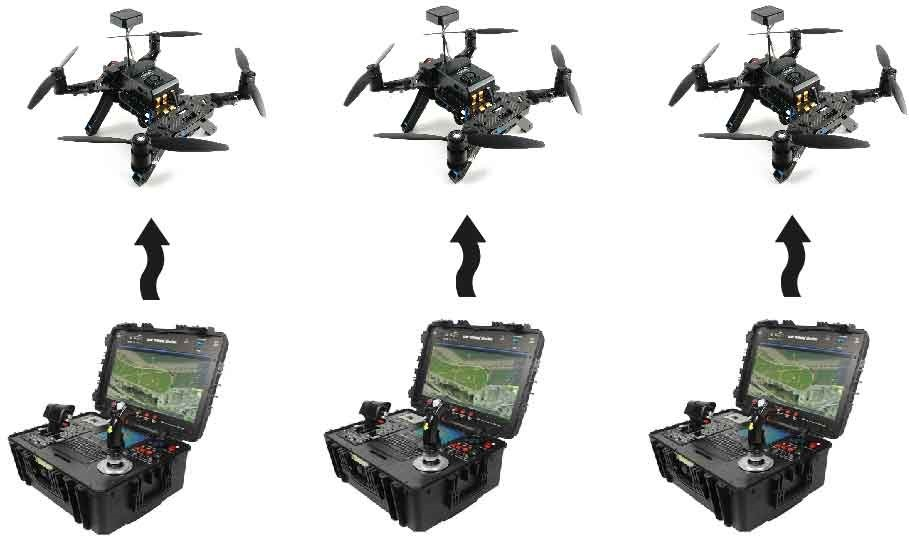
\includegraphics[width=60mm]{controlo_direto}
\caption{A arquitectura de controlo directo \label{fig:controlo_directo}}
\end{figure}

As GCSs podem ser implementadas de diferentes formas, podem ser implementadas através de uma antena Wi-Fi, que distribui o sinal de comando para os UAVs. Ou então, numa versão mais simples através de telecomando sendo que esta é opção a mais utilizada em captação de imagem e vídeo.

No entanto, como esta arquitectura é baseada num modelo de controlo mais centralizado possui algumas desvantagens tais como: 

\begin{itemize}
\item Se houver um ponto de falha, o sistema fica comprometido;
\item Nem todos os UAVs estão ligados à GCS a todo o instante, e assim os sinais de controlo podem não chegar ao drone;
\item E por fim, pode constituir um problema não só para comunicação mas também, para a segurança do sistema \cite{ImadJawhar2017}.
\end{itemize}

\subsection{Enxames de UAVs}

Um enxame de UAVs é capaz de formar redes expansíveis, para além das infraestruturas, que permitem o acesso dos nós terrestres. Ao beneficiar dos recursos de alta flexibilidade e de rápida provisão, a \textit{swarm} de UAVs é uma solução viável para recuperar a comunicação de forma rápida e eficaz, especialmente para cenários onde os recursos de comunicação são escassos ou inexistentes, como nos ambientes pós-desastre \cite{Shi2018}. 

Nesta arquitetura, as ligações d2d, \textit{drone-to-drone} são necessárias para fazer a comunicação entre os UAVs existentes no enxame. Num enxame de UAVs, existe uma hierarquia que é constituída por um líder e pelos seguidores. O líder é o UAV que recebe os comandos, e os seguidores são os que seguem a rota do líder e os comandos que lhe são passados por este.

\begin{figure}[H]
\centering
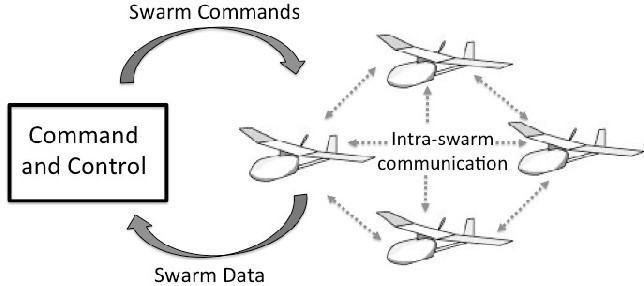
\includegraphics[width=10cm]{uav_swarm}
\caption{Diagrama de Controlo e Comando de um enxame UAV\label{fig:uav_swarm} }\cite{G.Madey2013}
\end{figure}

Esta topologia suporta não só a troca de mensagens de controlo entre os UAVs, de modo a prevenir colisões e a calcular rotas de voo,  bem como a transmissão dos dados para serem acedidos por outros UAVs. Existem UAVs específicos dentro do enxame que estão equipados com interfaces para comunicar com as infraestruturas ou satélites, estes estabelecem as \textit{gateways} entre o enxame e as outras redes.

Nos meios rurais ou em meios de pós-desastre onde as infraestruturas de cobertura são escassas, os enxames UAV são formados como infraestruturas aéreas temporárias para os veículos \cite{Shi2018}.

No exemplo citado no artigo \cite{He2018}, é estudada a possibilidade de um enxame de UAVs através do algoritmo proposto contar com vários líderes e também ao longo do tempo haver a possibilidade de aumentar o número de seguidores, a fim de reduzir o consumo de comunicação e melhorar a adaptabilidade do sistema e também a sua expansibilidade.

\subsection{Redes Mesh}

A rede \textit{mesh} sem fio consiste em nós de rádio organizados em uma topologia \textit{mesh} ou malha. São normalmente compostas por \textit{routers} e \textit{gateways mesh} que distribuem o sinal de \textit{Wi-Fi} igualmente por todos os pontos da rede.

Nestes cenários de rede, os \textit{routers} comunicam entre si e enviam sinal \textit{Wi-Fi} reciprocamente, bem como, para a área envolvente. Por exemplo, se um nó A quiser comunicar com o nó C irá utilizar o nó B que fica entre ambos para fornecer melhor possibilidade de comunicação. 

A este nó B, que se refere a um ponto intermediário, dá-se o nome de “salto” ou “\textit{hops}” da rede mesh. Cada um destes saltos, introduz um nível de atraso na rede, por isso é necessário que o número de saltos seja minimizado encontrando por exemplo o caminho mais direto entre os dois nós. No entanto, quando um dos \textit{routers} da rede \textit{mesh} fica \textit{offline} ou inutilizado o sinal consegue encontrar outros caminhos graças aos nós alternativos \cite{NetSpot}.

Nesta configuração de rede mesh encontra-se o projeto UAVNet referenciado pelo artigo \cite{Morgenthaler2012a}, que é uma \textit{framework} baseada numa altamente adaptável \textit{wireless mesh network}, WMN, que faz uso de UAVs pequenos equipados com \textit{wireless mesh nodes}, conectados aos UAV via porta série, de modo a poder interagir como uma \textit{mesh} em pleno ar.

\begin{figure}[H]
\centering
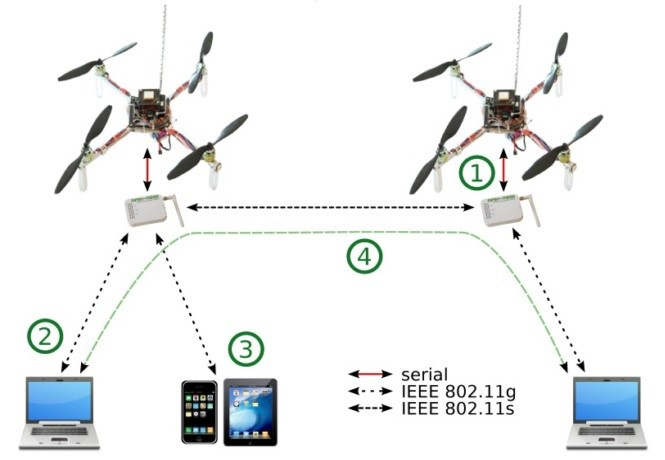
\includegraphics[width=10cm]{uav_net}
\caption{Exemplo de aplicação do \textit{UAVNet} \label{fig:uav_net} }\cite{Morgenthaler2012a}
\end{figure}

\subsection{Redes Ad-Hoc}

A tecnologia \textit{ad-hoc} permite a criação de redes de dispositivos móveis em áreas onde não existem infraestruturas de comunicações. Neste tipo de ligação não existe um nó central para onde todas as informações são enviadas pelos outros nós, fazendo com que não seja necessária a existência de um \textit{router} que faça a comunicação da rede com outros dispositivos externos. As ligações entre nós são independentes entre si, de maneira que, se uma falhar, seja por perda de conexão ou falha de algum dispositivo, todas as outras ligações continuam a funcionar \cite{DalloraMoraes2007}.

Como as redes \textit{ad-hoc} funcionam sem nenhuma infraestrutura é necessário que existam mecanismos de descoberta de rotas e encaminhamento de informação para isso estas redes recorrem a protocolos de rotas de dois tipos: os reativos e os pró-ativos.

Dentro dos protocolos reativos, que são protocolos que não tomam iniciativa de manter as rotas e apenas as determinam quando necessário fazendo \textit{flooding} de pedidos na rede. Este protocolo tem como vantagem o facto de usar recursos apenas quando é necessário, no entanto, inundam a rede com pedidos e introduzem atraso no inicio de envio do tráfego pois tem de ser primeiramente determinada a rota. Neste tipo de protocolos inclui-se o AODV definido pela norma RFC 3561, onde um determinado nó A envia um \textit{Route Request} para poder efetuar a comunicação com o nó B e recebe deste um \textit{Route Reply} de forma a indicar a rota mais próxima.

No caso dos protocolos pró-ativos, as rotas são construídas utilizando tráfego de controlo contínuo e mantém todas as rotas. Este processo tem como vantagem ter as rotas sempre disponíveis e mantém o tráfego de controlo constante. Um exemplo deste tipo de protocolo é o OLSR definido pela norma RFC 3626. Este protocolo implementa um sistema de deteção de ligação a nós vizinhos, através de mensagens \textit{HELLO}, efetua os pedidos de encaminhamento de forma otimizada através do mecanismo de MPR. Para além destes dois aspetos este protocolo envia mensagens de estado das ligações e cálculo de rotas \cite{Ricardoa}.

Em relação aos drones existem já estudos sobre as FANETs, que são redes \textit{ad-hoc} constituídas por UAVs, como se pode comprovar através do artigo \cite{Bekmezci2013a}. Um dos exemplos de rede ad-hoc com equipamentos UAV é o que está referenciado no artigo \cite{Brown2004} que fala de dois cenários de funcionamento, no primeiro o UAV atua como um nó de rádio  a proeminente que efetua a conexão de dos pontos de rádio terrestres desativados. No segundo cenário, a rede permite que os grupos de UAVs comuniquem entre si para estender o alcance operacional dos UAVs mais pequenos.

\begin{figure}[H]
\centering
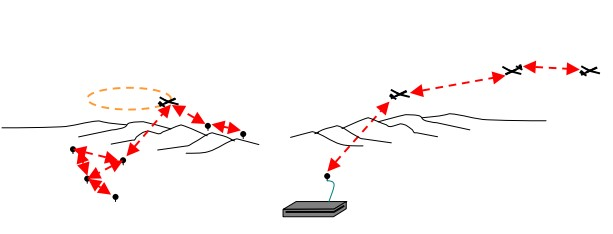
\includegraphics[width=10cm]{ad-hoc_protocols}
\caption{Figuras ilustrativas do cenário 1 (esquerda) e do cenário 2 (direita)  \label{fig:ad-hoc_protocols}}
\cite{Ricardoa}
\end{figure}

\subsection{Redes SD-UAV}

As redes definidas por software (SDN) são o novo paradigma de \textit{networking} no qual o \textit{hardware} de encaminhamento é dissociado das decisões de controlo. É uma tecnologia que promete simplificar a gestão da rede e permitir a inovação e evolução. A ideia principal é permitir que os software developers confiem nos recursos de rede da mesma maneira que fazem com os recursos de armazenamento e computação. Nas SDN, a inteligência da rede é centralizada logicamente nos controladores baseados em \textit{software} (plano de controlo) e os dispositivos de rede tornam-se simples dispositivos de encaminhamento de pacotes (plano de dados) que podem ser programados através de uma interface aberta \cite{Nunes2014} (ex. OpenFlow \cite{Leon-Garcia2015}, etc).

No artigo \cite{Secinti2018} é proposto um protocolo de gestão de uma rede aérea contruído em cima de uma arquitetura SDN. Neste projeto cada UAV torna-se num switch SDN que é controlado por diretivas enviadas por um controlador centralizado.

\begin{figure}[H]
\centering
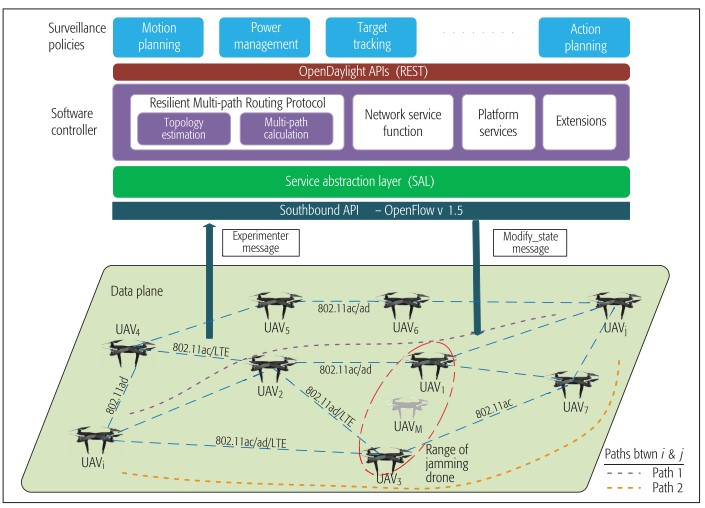
\includegraphics[width=10cm]{sd-uav_architecture}
\caption{Arquitetura SD-UAV proposta no artigo  \label{fig:sd-uav_architecture} }\cite{Secinti2018}
\end{figure}



\section{Áreas de aplicação das redes UAV}\label{sec:application}

Tal como dito em cima na secção \ref{sec:context}, os UAV e as suas redes tem várias utilidades tais como: escoltas militares, troca de mercadorias em algumas cidades, gestão do trânsito, fotografia aérea, segurança urbana. No entanto existem outros serviços e aplicações que estas podem operar.

\subsection{Retransmissão de Comunicação}

Os UAVs podem funcionar como nós de retransmissão, que conectam \textit{clusters} desconectados da rede \textit{ad hoc} móvel (MANET).  Nesse caso, os nós pertencentes a diferentes \textit{clusters} podem comunicar entre si utilizando um UAV, que pode ser colocado numa posição estratégica entre os dois. Por essa questão, um ou mais UAVs podem fornecer essa função em grandes MANETs, proporcionando eficiência de comunicação e flexibilidade. Adotando essa estratégia, pode se estender uma MANET numa área geográfica muito grande, onde os nós podem ter que ser agrupados em diferentes regiões devido aos requisitos de topologia de terrenos, localização de nós e mobilidade impostos pelo aplicação \cite{ImadJawhar2017}.

\subsection{Gateways de Rede}

Em áreas geográficas remotas ou áreas atingidas por desastres, um ou mais UAVs podem fornecer conectividade a redes de \textit{backbone}, infraestrutura de comunicação ou acesso à Internet agindo como nós de \textit{gateway}. Essa função pode desempenhar um papel essencial para restaurar a cobertura de telefone, Internet ou satélite desesperadamente necessária nesses locais. Essa conectividade pode apoiar esforços de busca e salvamento de vidas e reconstrução. Os UAVs podem ser implantados de maneira rápida e eficiente para executar essa tarefa de maneira muito dinâmica e económica \cite{ImadJawhar2017}.

\subsection{UAV-assisted Sensing}

As várias aplicações UAV requerem vários UAVs de colaboração para efetuar a deteção de uma área ou inspecionar uma infraestrutura utilizando um ou vários tipos de sensores como câmaras fotográficas, sensores de calores, leitores de radiação e monitores de gás. Essas aplicações exigem uma eficiência grande de comunicação de modo a permitir uma melhor deteção entre os vários UAVs. Alguns dos UAVs podem individualmente lidar com algumas das tarefas de deteção, uma solução eficiente para este problema passa por usar vários UAVs juntos na organização das operações e fazer uma colheita coletiva de informações mais precisas e confiáveis \cite{ImadJawhar2017}

\subsection{UAV-assisted Acting}

Em alguns casos, como fins agrícolas e militares, exigem dispositivos atuadores, como os UAVs. Nesse tipo de aplicações, vários UAVs podem colaborar entre si para realizar as tarefas necessárias. No caso da agricultura, vários UAVs poderiam trabalhar juntos para realizar a pulverização de grandes campos com pesticidas ou fazer distribuição rápida de sementes em grandes áreas \cite{ImadJawhar2017}.

\subsection{UAV-based data storage}

Apesar de algumas aplicações de UAVs enviem os dados recolhidos diretamente para a estação base, outros podem necessitar que os UAVs armazenem os a recolha de dados devido a três grandes motivos. A primeira é que os dados recolhidos necessitam de grande largura de banda de comunicação e os dados podem não estar sempre disponíveis para a transferência dos dados dos UAVs para a estação base. A segunda razão é que não existe a necessidade de enviar os dados recolhidos imediatamente para a estação logo após a recolha, pois a informação será usada e processada após a recolha. A terceira razão é que os dados recolhidos precisam de ser transferidos para a estação base somente após os dados serem processados e agregados instantaneamente durante a operação. Os UAVs podem ser homogéneos ou heterogéneos em termos de capacidade de armazenamento e capacidade de recolha de dados. Os UAVs podem recolher quantidades iguais ou diferentes de dados, dependendo claro do tipo de aplicação \cite{ImadJawhar2017}.

\subsection{UAV-based data processing}

Os UAVs podem ser equipados com unidades de processamento de última geração que podem ser utilizados por UAVs colaborativos para aplicações que precisam de processamento de alto desempenho, como processamento de imagem de alta resolução, processamento de vídeo, reconhecimento de padrões, fluxo de dados e planeamento de tarefas online. Uma tarefa de processamento de dados de alto desempenho pode ser obtida utilizando uma unidade computorizado num UAV ou várias unidades computorizadas disponíveis em vários UAVs. Neste último caso, precisa de ser efetivamente utilizada a abordagem de processamento distribuído pelos processadores disponíveis. Isso é geralmente muito importante se os UAVs estiverem a operar em zonas distantes das estações base e quando os resultados forem necessários no momento para acionar uma opção adequada. Por exemplo, num campo de batalha, um UAV pode precisar de identificar uma unidade inimiga que esteja próxima de algumas das suas unidades. Nesse caso o processamento de imagens e o reconhecimento de padrões são necessários para localizar o inimigo e tentar destruí-lo \cite{ImadJawhar2017}.

\section{Software de Controlo Open-Source}\label{chap:cs_opensource}

Nesta secção será analisada informação relativa tanto a software e protocolos open source existentes no mercado e que poderão a vir a ser utilizados na solução implementada.

\subsection{Papparazzi UAV}

O projeto Paparazzi UAV, fundado em 2003, é um projeto open source de hardware e software que abrange tanto a parte de software da estação terrena como os sistemas de pilotagem autónoma para os vários tipos de drones. Este projeto tem como principal foco o voo autónomo e o voo manual como um objetivo secundário \cite{TheFr2003}

\subsubsection{Arquitecturas Implementadas}

A nível das arquiteturas abordadas na secção acima este software é capaz de suportar todas as arquiteturas demonstradas acima com exceção das redes SD-UAV uma vez que ainda se encontra em fase de estudos. Estas implementações podem ser comprovadas pelos no artigos \cite{Remes2013,Bouachir2014a}.

\pagebreak
\subsubsection{Áreas de Aplicação}
Este software integra varias áreas de aplicação no entanto, as que mais se destacam nesta tecnologia são as seguintes:

\begin{itemize}
    \item Rede de Sensores;
    \item Investigação científica;
    \item Processamento de dados;
\end{itemize}

\subsubsection{Funcionalidades Protocolares de Comunicação e de Controlo}

A nível de funcionalidades protocolares de comunicações e controlo o Paparazzi UAV trabalha com alguns dos mais recentes protocolos de comunicação como o \textit{ZigBee(Xbee)}, /textit{Wi-Fi} e \textit{Bluetooth}\cite{TheFr2003}.

\subsection{ArduPilot}
O \textit{ArduPilot} é uma tecnologia que visa permitir a criação e o uso de sistemas de veículos não tripulados confiáveis e autónomos para o benefício pacífico de todos. É um projeto que atualmente pode ser descrito como uma \textit{suite} para um piloto automático \cite{ArduPilotCommunity}.

\subsubsection{Arquitecturas Implementadas}

As arquiteturas suportadas por esta tecnologia são as seguintes: controlo direto, enxames e também com mesh encontrando-se as áreas de ad-hoc e SD-UAV ainda em fase de desenvolvimento.

\subsubsection{Áreas de Aplicação}

Entre as áreas de aplicação desta tecnologia encontram-se:
\begin{itemize}
    \item {Mapeamento Aéreo;}
    \item Procura e Salvamento VTOL;
    \item Agricultura com os tratores automáticos;
    \item Controlo de veículos submarinos.
\end{itemize}

\subsubsection{Funcionalidades Protocolares de Comunicação e de Controlo}

A este nível de funcionalidades protocolares esta tecnologia é um pouco mais completa que a tecnologia apresentada anteriormente já que suporta não só o protocolo \textit{Wi-Fi} mas também suporta as tecnologias:
\begin{itemize}
    \item \textit{MAVLink} - é um protocolo de mensagens \textit{lightweight} para comunicação com drones (e entre componentes \textit{onboard} do drone). Segue um padrão de \textit{design} moderno híbrido de \textit{publish-subscriber} e ponto-a-ponto \cite{DronecodeProject}.
    \item CAN - \textit{Controller Area Network}
    \item UAVCAN - é um protocolo leve projetado para comunicação confiável em aplicações aeroespaciais e robóticas pelo barramento CAN \cite{UAVCANdevelopmentteam}.
\end{itemize}

\subsection{Dronecode}

A tecnologia Dronecode apresentação como uma solução \textit{full-stack} para os \textit{drones}, com soluções que vão desde a estação de controlo, GCS, até ao próprio \textit{drone} e aos seus sensores. Esta tecnologia criada sob a alçada da Fundação \textit{Linux} e que tem como objetivo promover o desenvolvimento dos drones contando com parceiros tais como a \textit{Qualcomm} e a \textit{Intel} \cite{DronecodeProject}.

\subsubsection{Arquitecturas Implementadas}

A nível de arquiteturas esta tecnologia é também uma das mais completas, tendo em conta os objectivos do projeto \textit{Dronecode} que é como diz em cima ser um dos parceiros para o desenvolvimento dos \textit{drones}. Por isso, esta tecnologia está apta a trabalhar com todas as arquiteturas referidas na secção \ref{sec:architectures}. 

\subsubsection{Áreas de Aplicação}

Nesta tecnologia as áreas de aplicação abrangidas são vastas, entre as quais destacam-se as seguintes:

\begin{itemize}
    \item Carga e Entrega - de pequenos pacotes como medicamentos;
    \item Inspeções aéreas - como por exemplo, mapeamento geográfico, inspeções em canteiros de obras e gasodutos, gestão da vida selvagem, gestão de fazendas etc;
    \item Entretenimento - competições e afins;
    \item Fotografia aérea;
    \item Busca, Salvamento e fiscalização - fiscalização de fronteiras;
    \item Exploração e Investigação - para fins académicos e científicos \cite{DronecodeProject}.
\end{itemize}

\subsubsection{Funcionalidades Protocolares de Comunicação e de Controlo}

A nível de funcionalidades protocolares de comunicação esta tecnologia utiliza também algumas das que já foram abordadas noutas tecnologias descritas em cima. Entre essas tecnologias estão o \textit{Wi-Fi}, o \textit{MAVLink} e o UAVCAN. Para além destas duas há ainda a destacar o RTPS, neste caso FastRTPS \cite{DronecodeProject}. O protocolo de comunicação RTPS que é uma \textit{framework publish subscrive} de alta performance que partilha a informação nos sistemas distribuidos utilizando um modelo desacoplado que se baseia em \textit{Publishers}, subscritores e \textit{Data Topics}\cite{EProsima}.

\subsection{LibrePilot}

O projecto \textit{open source} LibrePilot foi fundado em 2015. Este projecto foca-se na investigação e desenvolvimento de \textit{hardware} e \textit{software} para serem utilizados numa variedade de aplicações incluindo controlo de veículos e estabilização, UAVs e \textit{robots}. Um dos principais objectivos do projecto é conseguir arranjar um ambiente aberto e colaborativo e fazer dele a casa ideal para o desenvolvimento de ideias inovadoras \cite{LibrePilot}.

\subsubsection{Arquitecturas Implementadas}

Segundo a documentação desta tecnologia esta está mais virada para a arquitetura de controlo directo, focando-se muito na interação com \textit{smartphones} como estações de controlo através de uma \textit{app Android} que já se encontra disponível \textit{online}\cite{LibrePilot}.

\subsubsection{Áreas de Aplicação}

Esta tecnologia não é muito basta em termos de áreas de aplicação uma vez que na sua documentação e em foruns utilizados pela comunidade de developers apenas é referida a sua utilização para fotografia aérea \cite{LibrePilot}.

\subsubsection{Funcionalidades Protocolares de Comunicação e de Controlo}

Nas funcionalidades de comunicação e controlo para esta tecnologia encontra-se o protocolo \textit{MAVLink} já referida nesta secção e para além disso suporta também o protocolo MSP, que é um protocolo de comunicação desenvolvido pela \textit{MultiWii} desenhado para ser leve, genérico, eficiente e seguro \cite{MultiWii,MultiWiiForum}. 

\subsection{Comparação de soluções}

Nesta secção será disponibilizada uma tabela comparativa de todas as soluções apresentas nas sub-secções em cima.


%%%%%%%TABELA 1%%%%%%%%%%%%%%%%%%%%%%%%%%%%%%%%%%%%%%%%%%%%%%%%%%%%%%%%%%%%%%%%%%%%%%%
\begin{table}[H]
\caption{Comparação das várias opções de \textit{software}}
\begin{tabular}{l|c|c|c|}
\cline{2-4}
& \multicolumn{1}{l|}{Arquiteturas}  & \multicolumn{1}{l|}{Protocolos}  & \multicolumn{1}{l|}{Documentação} \\ \hline
\multicolumn{1}{|l|}{PapparazziUAV} & \textit{CD, SW, Mesh e Ad-Hoc}  & \textit{Xbee, Wi-Fi e Bluetooth} & Razoável \\ \hline
\multicolumn{1}{|l|}{ArduPilot}     & \textit{CD, SW, Mesh, Ad-Hoc e SD-UAV} & \textit{MAVLink, WiFi, CAN e UAVCAN}      & Boa                               \\ \hline
\multicolumn{1}{|l|}{Dronecode}     & Todas                                  & \textit{MAVLink, WiFi, UAVCAN e FastRTPS} & Muito Boa                         \\ \hline
\multicolumn{1}{|l|}{LibrePilot}    & CD                       & \textit{MAVLink e MSP}                    & Razoável                          \\ \hline
\end{tabular}
\end{table}
%%%%%%%%%%%%%%%%%%%%%%%%%%%%%%%%%%%%%%%%%%%%%%%%%%%%%%%%%%%%%%%%%%%%%%%%%%%%%%%%%%%%%%%%%%%%%%%%%




\chapter{Capítulo Exemplo}\label{chap:chap3}

Neste capítulo apresentam-se exemplos de formatação de figuras e
tabelas, equações e referências cruzadas.

Maecenas eleifend facilisis leo. Vestibulum et
mi. Aliquam posuere, ante non tristique consectetuer, dui elit
scelerisque augue, eu vehicula nibh nisi ac est. 
Suspendisse elementum sodales felis. Nullam laoreet fermentum urna. 

\section{Introdução}

Apresenta-se de seguida um exemplo de equação, completamente fora do contexto:
\begin{eqnarray}
CIF_1: \hspace*{5mm}F_0^j(a) &=& \frac{1}{2\pi \iota} \oint_{\gamma} \frac{F_0^j(z)}{z - a} dz\\
CIF_2: \hspace*{5mm}F_1^j(a) &=& \frac{1}{2\pi \iota} \oint_{\gamma} \frac{F_0^j(x)}{x - a} dx \label{eq:cif}
\end{eqnarray}

Na Equação~\ref{eq:cif} lorem ipsum dolor sit amet, consectetuer
adipiscing elit. Suspendisse tincidunt viverra elit. Donec tempus
vulputate mauris. Donec arcu. Vestibulum condimentum porta
justo. Curabitur ornare tincidunt lacus. Curabitur ac massa vel ante
tincidunt placerat. Cras vehicula semper elit. Curabitur gravida, est
a elementum suscipit, est eros ullamcorper quam, sed cursus velit
velit tempor neque. Duis tempor condimentum ante. Nam
sollicitudin. Vestibulum adipiscing, orci eu tempor dapibus, risus
sapien porta metus, et cursus leo metus eget nibh. 

Pellentesque rutrum, sapien at viverra facilisis, metus eros blandit
sem, quis dictum erat metus eget erat. Vivamus malesuada dapibus
nulla. Maecenas nec purus. Suspendisse auctor mattis augue. Phasellus
enim nisi, iaculis sit amet, pellentesque a, iaculis in, dui. Integer
risus. 

\section{Secção Exemplo}

A arquitectura do visualizador assenta sobre os seguintes conceitos
base~\citep{kn:ZPMD97}: 

\begin{itemize}
\item \textbf{Componentes} --- Suspendisse auctor mattis augue \emph{push};
\item \textbf{Praesent} --- Sit amet sem maecenas eleifend facilisis leo;
\item \textbf{Pellentesque} --- Habitant morbi tristique senectus et netus.
\end{itemize}

\subsection{Exemplo de Figura}

É apresentado na Figura~\ref{fig:arch} da página~\pageref{fig:arch} um
exemplo de figura flutuante que deverá ficar no topo da página.

\begin{figure}[t]
  \begin{center}
    \leavevmode
    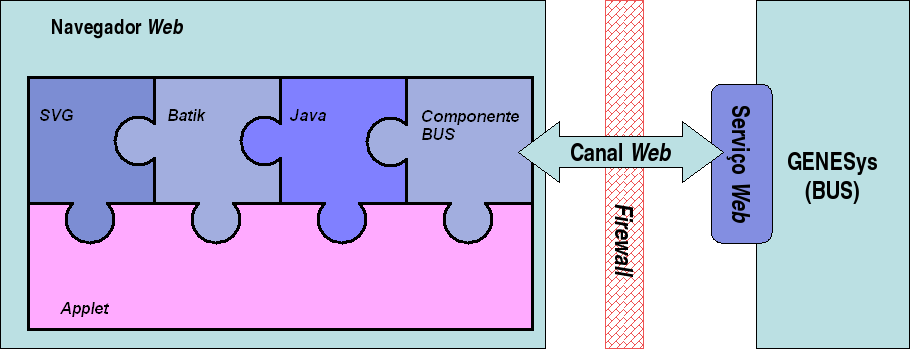
\includegraphics[width=0.86\textwidth]{puzzle}
    \caption{Arquitectura da Solução Proposta}
    \label{fig:arch}
  \end{center}
\end{figure}

Loren ipsum dolor sit amet, consectetuer adipiscing elit. 
Praesent sit amet sem. Maecenas eleifend facilisis leo. Vestibulum et
mi. Aliquam posuere, ante non tristique consectetuer, dui elit
scelerisque augue, eu vehicula nibh nisi ac est. Suspendisse elementum
sodales felis. Nullam laoreet fermentum urna. 

Duis eget diam. In est justo, tristique in, lacinia vel, feugiat eget,
quam. Pellentesque habitant morbi tristique senectus et netus et
malesuada fames ac turpis egestas. Fusce feugiat, elit ac placerat
fermentum, augue nisl ultricies eros, id fringilla enim sapien eu
felis. Vestibulum ante ipsum primis in faucibus orci luctus et
ultrices posuere cubilia Curae; Sed dolor mi, porttitor quis,
condimentum sed, luctus in. 

\subsection{Exemplo de Tabela}

É apresentado na Tabela~\ref{tab:exemplo} um exemplo de tabela
flutuante que deverá ficar no topo da página.

\begin{table}[t]
  \centering
  \caption{Tabela Exemplo}
\begin{tabular}{|c|r@{.}lr@{.}lr@{.}l||r|}
	\hline
\multicolumn{8}{|c|}
	{\rule[-3mm]{0mm}{8mm}Iteração $k$ de $f(x_n)$} \\
\textbf{\em k}
	& \multicolumn{2}{c}{$x_1^k$}
	& \multicolumn{2}{c}{$x_2^k$}
	& \multicolumn{2}{c||}{$x_3^k$}
	& comentários \\ \hline \hline
0   & -0&3                 & 0&6                 &  0&7   & - \\
1   &  0&47102965 & 0&04883157 & -0&53345964  & $\delta<\epsilon$ \\
2   &  0&49988691 & 0&00228830 & -0&52246185  & $\delta < \varepsilon$ \\
3   &  0&49999976 & 0&00005380 & -0&523656   &   $N$ \\
4   &  0&5                 & 0&00000307 & -0&52359743  & \\
\vdots	& \multicolumn{2}{c}{\vdots}
	& \multicolumn{2}{c}{$\ddots$}
	& \multicolumn{2}{c||}{\vdots}  & \\
7   &  0&5   & 0&0    & \textbf{-0}&\textbf{52359878}
		 & $\delta<10^{-8}$ \\ \hline
\end{tabular}
  \label{tab:exemplo}
\end{table}

Loren ipsum dolor sit amet, consectetuer adipiscing elit. 
Praesent sit amet sem. Maecenas eleifend facilisis leo. Vestibulum et
mi. Aliquam posuere, ante non tristique consectetuer, dui elit
scelerisque augue, eu vehicula nibh nisi ac est. Suspendisse elementum
sodales felis. Nullam laoreet fermentum urna. 

Duis eget diam. In est justo, tristique in, lacinia vel, feugiat eget,
quam. Pellentesque habitant morbi tristique senectus et netus et
malesuada fames ac turpis egestas. Fusce feugiat, elit ac placerat
fermentum, augue nisl ultricies eros, id fringilla enim sapien eu
felis. Vestibulum ante ipsum primis in faucibus orci luctus et
ultrices posuere cubilia Curae; Sed dolor mi, porttitor quis,
condimentum sed, luctus in. 

\section{Secção Exemplo}

Loren ipsum dolor sit amet, consectetuer adipiscing elit. 
Praesent sit amet sem. Maecenas eleifend facilisis leo. Vestibulum et
mi. Aliquam posuere, ante non tristique consectetuer, dui elit
scelerisque augue, eu vehicula nibh nisi ac est. Suspendisse elementum
sodales felis. Nullam laoreet fermentum urna. 

Duis eget diam. In est justo, tristique in, lacinia vel, feugiat eget,
quam. Pellentesque habitant morbi tristique senectus et netus et
malesuada fames ac turpis egestas. Fusce feugiat, elit ac placerat
fermentum, augue nisl ultricies eros, id fringilla enim sapien eu
felis. Vestibulum ante ipsum primis in faucibus orci luctus et
ultrices posuere cubilia Curae; Sed dolor mi, porttitor quis,
condimentum sed, luctus in. 

\section{Resumo}

Pellentesque habitant morbi tristique senectus et netus et
malesuada fames ac turpis egestas. Fusce feugiat, elit ac placerat
fermentum, augue nisl ultricies eros, id fringilla enim sapien eu
felis. Vestibulum ante ipsum primis in faucibus orci luctus et
ultrices posuere cubilia Curae; Sed dolor mi, porttitor quis,
condimentum sed, luctus in. 

\chapter{Sistema Proposto}\label{chap:chap4}
\chapter{Conclusões e Trabalho Futuro} \label{chap:concl}

Proin sed justo eu sapien eleifend elementum. Pellentesque
habitant morbi tristique senectus et netus et malesuada fames ac
turpis egestas. Vivamus quam lacus, pharetra vel, aliquam vel,
volutpat sed, nisl. 

\section{Satisfação dos Objetivos}

Lorem ipsum dolor sit amet, consectetuer adipiscing elit. Etiam non
felis sed odio rutrum ultrices. Donec tempor dolor. Vivamus justo
neque, tempus id, ullamcorper in, pharetra non, tellus. Praesent eu
orci eu dolor congue gravida. Sed eu est. Donec pulvinar, lectus et
eleifend volutpat, diam sapien sollicitudin arcu, a sagittis libero
neque et dolor. Nam ligula. Cras tincidunt lectus quis nunc. Cras
tincidunt congue turpis. Nulla pede velit, sagittis a, faucibus vitae,
porttitor nec, ante. Nulla ut arcu. Cras eu augue at ipsum feugiat
hendrerit. Proin sed justo eu sapien eleifend elementum. Pellentesque
habitant morbi tristique senectus et netus et malesuada fames ac
turpis egestas. Vivamus quam lacus, pharetra vel, aliquam vel,
volutpat sed, nisl. 

Nullam erat est, vehicula id, tempor non, scelerisque at,
tellus. Pellentesque tincidunt, ante vehicula bibendum adipiscing,
lorem augue tempor felis, in dictum massa justo sed metus. Suspendisse
placerat, mi eget molestie sodales, tortor ante interdum dui, ac
sagittis est pede et lacus. Duis sapien. Nam ornare turpis et
magna. Etiam adipiscing adipiscing ipsum. Fusce sodales nisl a
arcu. Cras massa leo, vehicula facilisis, commodo a, molestie
faucibus, metus. Suspendisse potenti. Duis sagittis. Donec porta. Sed
urna. Maecenas eros. Vivamus erat ligula, pharetra sit amet, bibendum
et, fermentum sed, dolor. Nullam eleifend condimentum nibh. Integer
leo nibh, consequat eget, mollis et, sagittis ac, felis. Duis viverra
pede in pede. Phasellus molestie placerat leo. Praesent at tellus a
augue congue molestie. Proin sed justo eu sapien eleifend
elementum. Pellentesque habitant morbi tristique senectus et netus et
malesuada fames ac turpis egestas. 

\section{Trabalho Futuro}

Lorem ipsum dolor sit amet, consectetuer adipiscing elit. Aliquam
tempor tristique risus. Suspendisse potenti. Fusce id eros. In eu
enim. Praesent commodo leo. Nullam augue. Pellentesque tellus. Integer
pulvinar purus a dui convallis consectetuer. In adipiscing, orci vitae
lacinia semper, sapien elit posuere sem, ac euismod ipsum elit tempus
urna. Aliquam erat volutpat. Nullam suscipit augue sed
felis. Phasellus faucibus accumsan est. 

Aliquam felis justo, facilisis sit amet, bibendum ut, tempus ac,
dolor. Sed malesuada. Nunc non massa. In erat. Nulla
facilisi. Phasellus blandit, est in accumsan cursus, libero augue
elementum leo, vitae auctor mauris nisl ac tortor. Cras porttitor
ornare elit. Fusce at lorem. Sed lectus tortor, vestibulum id, varius
a, condimentum nec, lectus. Maecenas in nisi et magna pretium
aliquam. Pellentesque justo elit, feugiat nec, tincidunt a, dignissim
vel, ipsum. Sed nunc. Vestibulum ante ipsum primis in faucibus orci
luctus et ultrices posuere cubilia Curae; Aliquam tempus rhoncus
leo. Donec neque quam, cursus sit amet, ultricies varius, semper non,
pede. Donec porttitor. Sed aliquet feugiat elit.  

\vspace*{12mm}

Lorem ipsum dolor sit amet, consectetuer adipiscing elit. Phasellus
tellus pede, auctor ut, tincidunt a, consectetuer in, felis. Mauris
quis dolor et neque accumsan pellentesque. Donec dui magna,
scelerisque mattis, sagittis nec, porta quis, nulla. Vivamus quis
nisl. Etiam vitae nisl in diam vehicula viverra. Sed sollicitudin
scelerisque est. Nunc dapibus. Sed urna. Nulla gravida. Praesent
faucibus, risus ac lobortis dignissim, est tortor laoreet mauris,
dictum pellentesque nunc orci tincidunt tellus. Nullam pulvinar, leo
sed vestibulum euismod, ante ligula elementum pede, sit amet dapibus
lacus tortor ac nisl. Morbi libero. Integer sed dolor ac lectus
commodo iaculis. Donec ut odio.  


%%----------------------------------------
%% Appendices
%%----------------------------------------
%% Comment next 2 commands if numbered appendices are not used
\appendix
%%%----------------------------------------
%% Appendix 1
%%----------------------------------------

\chapter{Lorem Ipsum} \label{ap1:Lorem}


%%%----------------------------------------
%% Appendix 2
%%----------------------------------------
\chapter{Lorem Ipsum} \label{ap2:Lorem}



%%----------------------------------------
%% Final materials
%%----------------------------------------

%% Bibliography
%% Comment the next command if BibTeX file not used, 
%% Assumes that bibliography is in 'myrefs.bib'
%% plainnat-pt.bst is used by default
%\PrintBib{Bibliography/myrefs}
\bibliographystyle{ieeetr}
\bibliography{Bibliography/myrefs}

%% Index
%% Uncomment next command if index is required, 
%% don't forget to run ``makeindex tese'' command
%\PrintIndex
\end{document}